\documentclass[a4paper, 11pt]{article}
\usepackage{preamble}

\usepackage{listings}


\newcommand{\website}{\url{http://pierre.gaillard.me/teaching/mva}}
\newcommand{\email}{pierre.gaillard@inria.fr}

\lstset{language=python,basicstyle={\ttfamily}}

\usepackage{newfloat}
\DeclareFloatingEnvironment{algo}
\renewcommand{\algoname}{Algorithm}

\DeclareFloatingEnvironment{setting}
\renewcommand{\settingname}{Setting}

\newcommand{\indic}{\mathds{1}}

\makeatletter
\newenvironment{fullwidth}
    {\par
     \setlength{\@totalleftmargin}{0pt}%
     \setlength{\linewidth}{\hsize}%
     \list{}{\setlength{\leftmargin}{0pt}}
     \item\relax}
    {\endlist}
\makeatother

\newenvironment{solution}{\vspace{2mm}\begin{fullwidth} \textbf{Solution:}}{\end{fullwidth}\vspace{2mm}}

\begin{document}

\doctype{Homework}
\coursetitle{Sequential Learning}
\semester{MVA 2020}
\instructor{Pierre Gaillard}
\student{Céline Moucer, Antoine Moulin}
\worknumber{}
\workdate{March 6}

\maketitle

This homework is due by {\bfseries Friday March 6, 2020}. It is to be returned by email to \href{mailto:\email}{\email} {\bfseries as a pdf file} (not a jupyter notebook). The code can be done in any langage (\texttt{python}, \texttt{R}, \texttt{matlab},\dots) but the results and the figures must be included into the pdf report. 

\medskip
Most questions require a proper mathematical justification or derivation (unless otherwise stated), but most questions can be answered concisely in just a few lines. No question should require lengthy or tedious derivations or calculations.


\section*{Part 1. Link between online learning and game theory}

We consider the sequential version of a two-player zero-sum games between a player and an adversary. 
\begin{setting}[ht!]
\begin{center}
\fbox{
    \begin{minipage}{.95\textwidth}
		Let $L \in [-1,1]^{M \times N}$ be a loss matrix.  \\[2pt]
        At each round $t=1,\dots,T$
        \begin{itemize}
            \item The player choose a distribution $p_t \in \Delta_{M} := \{p \in [0,1]^M, \sum_{i=1}^M p_i = 1\}$
            \item The adversary chooses a distribution $q_t \in \Delta_N$
            \item The actions of both players are sampled $i_t \sim p_t$ and $j_t \sim q_t$
            \item The player incurs the loss $L(i_t,j_t)$ and the adversary the loss $-L(i_t,j_t)$. 
        \end{itemize}
    \end{minipage}}
\end{center}

\caption{Setting of a sequential two-player zero sum game}
\label{fig:setting}
\end{setting}

\begin{enumerate}
	\item Recall $M$, $N$ and a loss matrix $L \in [-1,1]^{M\times N}$ that corresponds to the game ``Rock paper scissors''\footnote{This is a common game where two players choose one of 3 options: (Rock, Paper, Scissors). The winner is decided according to the following: Rock crushes scissors, Paper covers Rock, Scissors cuts paper}.
	
    \begin{solution}
For the game "Rock paper scissors", the player and the adversary have three possible actions, so:

\begin{equation*}
        \boxed{N=M=3}
\end{equation*}

and the loss is (in a basis "Rock paper scissors"):

\begin{equation*}
            \boxed{L = \begin{pmatrix}
       0 & 1 & -1 \\
       -1 & 0 & 1 \\
       1 & -1 & 0
    \end{pmatrix}}
        \end{equation*}
    \end{solution}
\end{enumerate}

\paragraph{Full information feedback}
In this part, we assume that both players know the matrix $L$ in advance and can compute $L(i,j)$ for any $(i,j)$. 

\begin{enumerate}[resume]
	\item \emph{Implementation of \lstinline{EWA}.} 
	\begin{enumerate}[label=(\alph*)] 
		\item In order to implement the exponential weight algorithm, you need a way to sample from the exponential weight distribution. Implement the function \lstinline{rand_weighted} that takes as input a probability vector $p \in \Delta_M$ and uses a single call to \lstinline{rand()} to return $X \in [M]$ with $P(X = i) = p_i$.
		
	    \begin{solution}
    See code.
        \end{solution}


		\item Define a function \lstinline{EWA_update} that takes as input a vector $p_t \in \Delta_M$ and a loss vector $\ell_t \in [-1,1]^M$ and return the updated vector $p_{t+1} \in \Delta_M$ defined for all $i \in [M]$ by
		\begin{equation*}
			p_{t+1}(i) = \frac{p_t(i) \exp(-\eta \ell_t(i))}{\sum_{j=1}^M p_t(j) \exp(-\eta \ell_t(j))} \,.
		\end{equation*}
		
	    \begin{solution}
    See code.
        \end{solution}
	\end{enumerate}

	\item \emph{Simulation against a fixed adversary.} Consider the game ``Rock paper scissors'' and assume that the adversary chooses $q_t = (1/2, 1/4, 1/4)$ and samples $j_t \sim q_t$ for all rounds $t \geq 1$. 
	\begin{enumerate}[label=(\alph*)]
		\item What is the loss $\ell_t(i)$ incurred by the player if he chooses action $i$ at time $t$? Simulate an instance of the game for $t = 1,\dots, T= 100$ for $\eta = 1$.
		
	    \begin{solution}
    The loss incurred by the player if he chooses action i at time t is:
    
    \begin{equation*}
        \boxed{\ell_t(i)=L(i,j_t)}
    \end{equation*}
        \end{solution}
		
		
 		\item Plot the evolution of the weight vectors $p_1,p_2,\dots,p_T$. What seems to be the best strategy against this adversary?
 		
	    \begin{solution}
\begin{figure}[h!]
\begin{center}
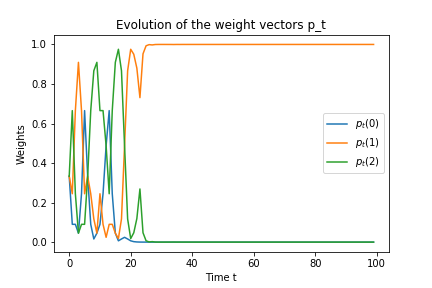
\includegraphics[height=170 pt]{image1/q3b_weights.png} 
\end{center}
\caption{Evolution of the weight vectors from the EWA algorithm for $\eta = 1$ and $T = 100$, as a function of $t$.}
\end{figure}
From this figure, we can conclude that the best strategy against this adversary is to play the action 1 all the time. It is indeed quite coherent with the game, since the action 1 (paper) wins over the action 0 (rock), which is the most played since the adversary chooses it half of the time ($q_t = (1/2,1/4,1/4)$).
        \end{solution}
 		
 		
 		\item Plot the average loss $\bar \ell_t = \frac{1}{t} \sum_{s=1}^t \ell(i_s,j_s)$ as a function of $t$.
 		
	    \begin{solution}
	    \begin{figure}[h!]
\begin{center}
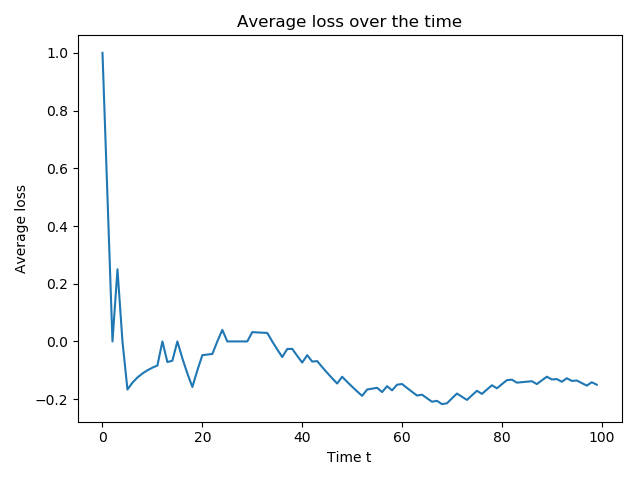
\includegraphics[height=170 pt]{image1/q3c_average_loss.png} 
\end{center}
\caption{Average loss for EWA algorithm for $\eta = 1$ and $T = 100$, as a function of $t$.}
\end{figure}
We notice that the average loss tends to be negative, meaning the player is winning in the long run. It shows that the EWA strategy is working against a non-adaptative adversary. The limit seems to be $-0.2$, which corresponds to the expected loss when the probability distributions are $p = \br{0, 1, 0}$ and $q = \br{1/2, 1/4, 1/4}$.
        \end{solution}
 		
 		
 		\item Plot the cumulative regret.

	    \begin{solution}
Let us plot the cumulative regret compared to: 
\begin{itemize}
    \item The optimal bound (for the optimal $\eta$): $f(t)=2\sqrt{tlog(3)}$.
    \item The actual bound: $f(t) = \eta t + \frac{log(3)}{\eta}$.
\end{itemize}
\begin{figure}[h!]
\centering
\begin{subfigure}{.47\textwidth}
  \centering
  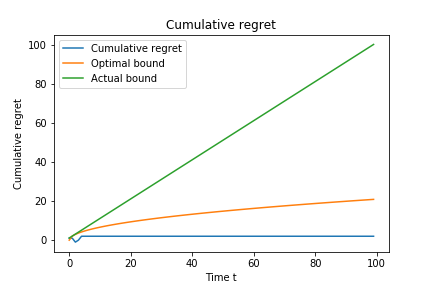
\includegraphics[height=150pt]{image1/q3d_regrets.png}
  \caption{Cumulative regret of the EWA algorithm for $\eta = 1$ and $T = 100$, as a function of $t$, compared with the real bound and its optimal one.}
  \label{fig:sub1}
\end{subfigure}%
\hspace{2mm}
\begin{subfigure}{.47\textwidth}
  \centering
  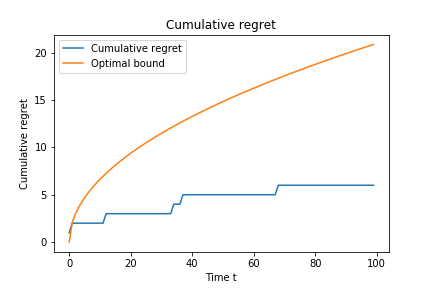
\includegraphics[height=150pt]{image1/q3d_regrets_bis.png}
  \caption{Cumulative regret of the EWA algorithm for $\eta = 1$ and $T=100$, as a function of t, compared with the optimal bound.}
  \label{fig:sub2}
\end{subfigure}%
\caption{Cumulative regret of the EWA.}
\label{fig:cum-regrets}
\end{figure}
The cumulative regret is below the actual and the optimal bound, even with a non optimal value of $\eta$.
        \end{solution}
 		
 		
 		\item To see if the algorithm is stable, repeat the simulation $n = 10$ times and plot the average loss $(\bar \ell_t)_{t\geq 1}$ obtained in average, in maximum and in minimum over the $n$ simulations.
 		
	    \begin{solution}
	    The plot is given in figure \ref{fig:loss-measures} and shows that the algorithm is stable: the minimum and the maximum loss are both concentrating around the average loss, what indicates a low variance average loss when t increases.
	\begin{figure}   
    \begin{center}
    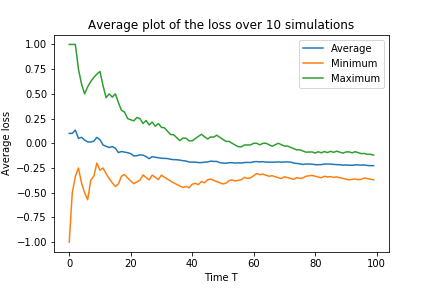
\includegraphics[height=150 pt]{image1/q3e_average_simulations.png}
    \end{center}
    \caption{Average loss for EWA over 10 simulations for $\eta = 1$ and $T=100$, as a function of $t$.}
    \label{fig:loss-measures}
    \end{figure}
        \end{solution}
 	
 		\item Repeat one simulation for different values of learning rates $\eta \in \{0.01,0.05,0.1,0.5,1\}$ and plot the final regret as a function of $\eta$. What are the best $\eta$ in practice and in theory.
 		
	    \begin{solution}
    \begin{figure}[h!]  
    \begin{center}
    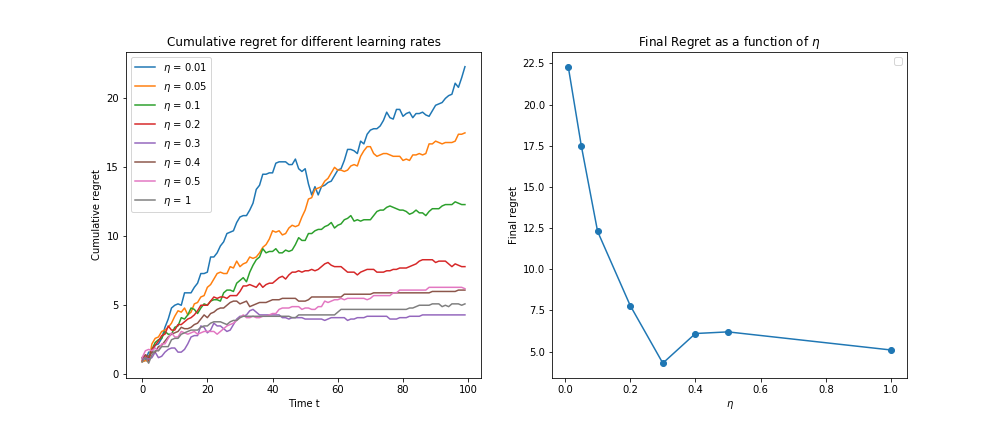
\includegraphics[height=170 pt]{image1/q3f_eta_variations_100.png}
    \end{center}
    \caption{Average loss for EWA for different values of $eta$ and $T=100$, as a function of $t$.}
    \end{figure}
    
    \begin{figure}[h!]   
    \begin{center}
    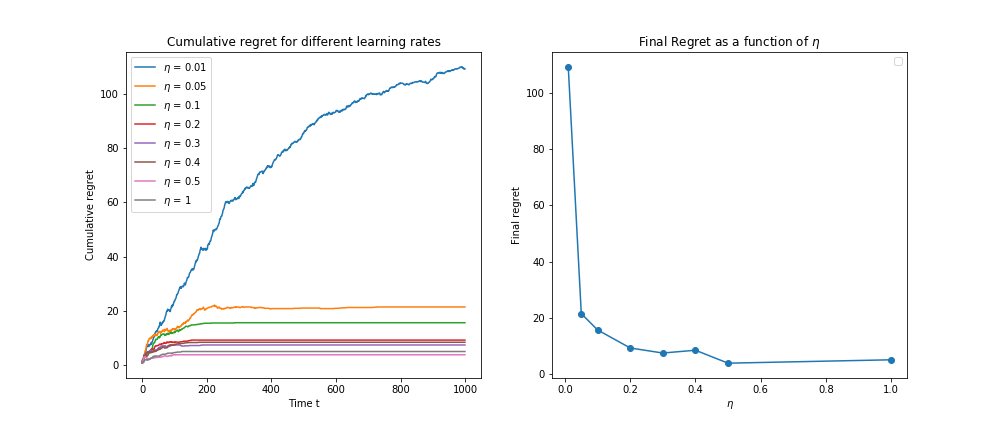
\includegraphics[height=170 pt]{image1/q3f_eta_variations_1000.png}
    \end{center}
    \caption{Average loss for EWA for different values of $eta$ and $T=1000$, as a function of $t$.}
    \end{figure}
        \end{solution}

The best values for $\eta$ are obtained for $\eta \in [0.2,1]$. We performed the simulation for T=100, and for T=1000, since the final regrets are used to compare $\eta$. In theory, the best value for $\eta$ is achieved with: 
\begin{equation*}
    \eta = \sqrt{\frac{log(M)}{T}}
\end{equation*}

Thus, $\eta \approx 0.03$ if $T=1000$, and $\eta \approx 0.1$ for $T=100$. However, we reach better results for higher values of $\eta$. Indeed, the plot in figure \ref{fig:cum-regrets} showed that the optimal bound is not tight. We could explain this phenomenon with the quite simple structure of the problem. Lower values of $\eta$ allow to explore more first. But here, since the action is not adaptative, higher values of $\eta$ only allows to converge quicker to action 1 (question (3.b)), and keep the loss slow in the first plays.
	\end{enumerate}

	\item \emph{Simulation against an adaptive adversary.} Repeat the simulation of question 3) when the adversary is also playing EWA with learning parameters $\eta = 0.05$.  

	\begin{enumerate}[label=(\alph*)]
		\item Plot $\frac{1}{t} \sum_{s=1}^t \ell(i_s,j_s)$ as a function of $t$. 
		
	    \begin{solution}
    In this question, the adversary becomes adaptative with EWA updates and $\eta_2=0.05$, the player still follows EWA updates with $\eta_1 = 0.05$.
     \begin{figure}[h!]  
    \begin{center}
    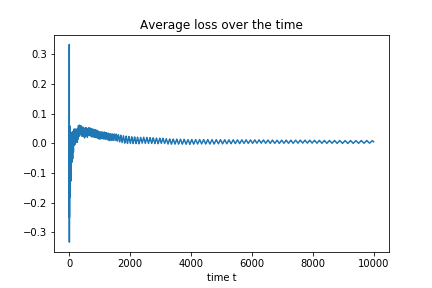
\includegraphics[height=150 pt]{image1/q4a_average_loss.png}
    \end{center}
    \caption{Average loss for an adaptative EWA adversary as a function of $t$, with $T = 10000$, $\eta_1 = 0.05$, and $\eta_2 = 0.05$.}
    \end{figure}
    
    The average loss converges to $0$. This is coherent with the course (if the adversary follows a regret minimization algorithm, the average loss converges almost surely). Besides, since the losses are symmetric for the player and its adversary, the value of the limit is also coherent.
        \end{solution}

		\smallskip
		It is possible to show that if both players  play according to a regret minimizing strategy the cumulative
loss of the player converges to the value of the game
		\begin{equation*}
			V = \min_{p \in \Delta_M} \max_{q \in 
\Delta_q} \ p^\top L q \,.
		\end{equation*}
		\item Define $\bar p_t = \frac{1}{t} \sum_{s=1}^t p_s$. Plot in log scale $\|\bar p_t - (1/3,1/3,1/3)\|_2$ as a function of $t=1,\dots,10\,000$. 
		
	    \begin{solution}
\begin{figure}
\begin{center}
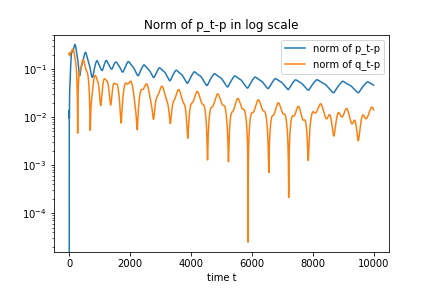
\includegraphics[height=170 pt]{image1/EWA_norm.png} 
\end{center}
\caption{Plot of $||\bar{p_t}-(1/3,1/3,1/3)||_2$ and $||\bar{q_t}-(1/3,1/3,1/3)||_2$, for $\eta=0.05$ and $T=10000$}
\end{figure}

The norm $\|\bar p_t - (1/3,1/3,1/3)\|_2$ converges to $0$, and oscillates while decreasing, and so does $\|\bar q_t - (1/3,1/3,1/3)\|_2$. This is again coherent with the Nash equilibrium : both player follows a minimization regret algorithm, and thus tend to have a uniform action.
        \end{solution}

		\smallskip
		It is possible to show that $(\bar p_t, \bar q_t)_{t\geq 1}$ converges almost surely to a Nash equilibrium of the game. This means that if $p\times q$ is a Nash equilibrium, none of the players should change is strategy if the other player does not change hers. 
	\end{enumerate}
\end{enumerate}

\paragraph{Bandit feedback}
Now, we assume that the players do not know the game in advance but only observe the performance $L(i_t,j_t)$ (that we assume here to be in $[0,1]$) of the actions played at time $t$. They need to learn the game and adapt to the adversary as one goes along.

\begin{enumerate}[resume]
    \item \emph{Implementation of \lstinline{EXP3}}. Since both players are symmetric, we focus on the first player. 
    \begin{enumerate}[label=(\alph*)]
    	\item Implement the function \lstinline{estimated_loss} that takes as input the action $i_t \in [M]$ played at round $t\geq 1$ and the loss $L(i_t,j_t)$ suffered by the player and return the vector of estimated loss $\widehat \ell_t \in \R_+^M$ used by \lstinline{EXP3}.
	
	    \begin{solution}
    See the code.
        \end{solution}
	
	
	    \item Implement the function \lstinline{EXP3_update} that takes as input a vector $p_t \in \Delta_M$, the action $i_t \in [M]$ played by the player and the loss $L(i_t,j_t)$ and return the updated weight vector $p_{t+1} \in \Delta_M$.
	    
	    \begin{solution}
    See the code.
        \end{solution}
    \end{enumerate}

    \item Repeat Questions 3.a) to 3.f) with \lstinline{EXP3} instead of \lstinline{EWA}.
    
    \begin{solution}
    When using \lstinline{EXP3} instead of \lstinline{EWA}, we observe that even though the algorithm takes more time to learn the optimal strategy, we obtain similar results for questions 3.a) to 3.f). Indeed, although the information is now incomplete, the game is simple enough so the algorithm can learn to counter a fixed adversary and have a low regret. To see the plots, one can just run the script \lstinline{main.py}. Here are some of them in figure \ref{fig:cum-regrets}.
    
    \begin{figure}[!h]
\centering
\begin{subfigure}{.28\textwidth}
  \centering
  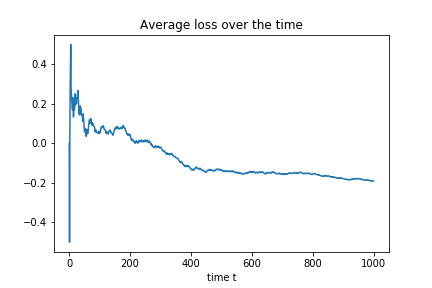
\includegraphics[height=100pt]{image1/EXP3/EXP3_average_loss.png}
  \caption{Cumulative regret of EXP3, for $\eta = 1, T = 1000$, as a function of $t$, compared with the real and optimal bounds.}
  \label{fig:sub1}
\end{subfigure}%
\hspace{.5mm}
\begin{subfigure}{.28\textwidth}
  \centering
  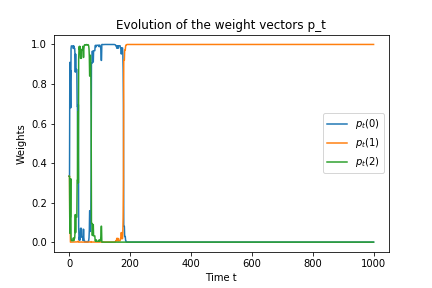
\includegraphics[height=100pt]{image1/EXP3/EXP3_proba.png}
  \caption{Evolution of the weight vectors for EXP3, $\eta = 1$ and $T = 1000$, as a function of $t$.}
  \label{fig:sub2}
\end{subfigure}%
\hspace{.5mm}
\begin{subfigure}{.28\textwidth}
  \centering
  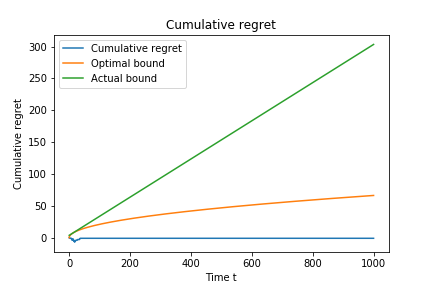
\includegraphics[height=100pt]{image1/EXP3/EXP3_comparison.png}
  \caption{Average loss for EXP3 over 10 simulations, for $\eta=1$ and $T=1000$, as a function of t}
  \label{fig:sub1}
\end{subfigure}%
\caption{}
\label{fig:cum-regrets}
\end{figure}

We observe the same behavior for the weight vectors and the average loss as for the EWA algorithm. The cumulative regret is again under the optimal bound even if the $\eta$ value is not the optimal one.

\begin{figure}[!h]
\begin{center}
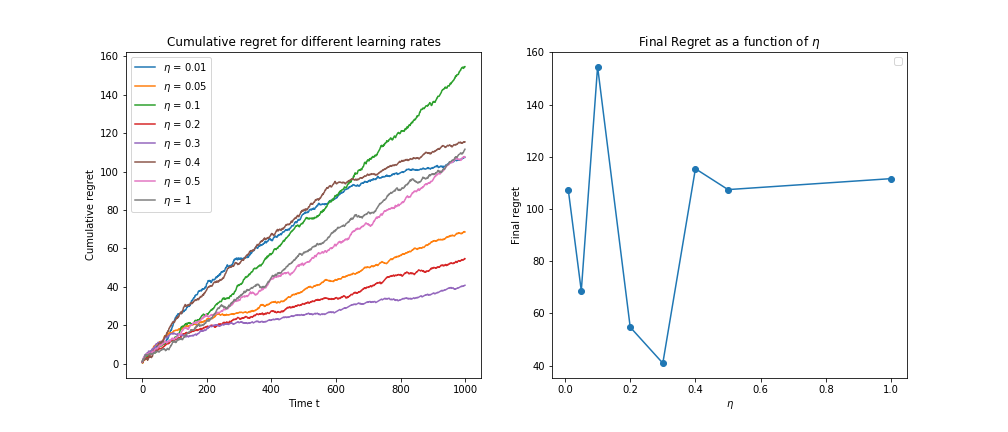
\includegraphics[height=190 pt]{image1/EXP3/EXP3_comparison_eta.png} 
\end{center}
\caption{Average loss for EXP3 as a function of t, with $\eta$ varying on a grid, and $T=1000$.}
\end{figure}

This comparison highlights the differences between EWA and EXP3. Indeed, the best cumulative regret seems to be much higher than on figure 6 for EWA, and the value of $\eta$ more discriminant. Even if the best $\eta$ is again around 0.3, small variations around this values induces big differences in the cumulative regret. Thus, EXP3 is less stable than EWA when considering the optimal $\eta$ value.
    \end{solution}

    \item Repeat Question 4.a) and 4.b) with \lstinline{EXP3} instead of \lstinline{EWA}.
    
    \begin{solution}
    As previously, we can obtain a loss of $0$, but \lstinline{EXP3} is less stable than \lstinline{EWA}. Indeed, although we have a loss of $0$ as shown in figure \ref{fig:q7a}, the strategy obtained is not the uniform distribution but a constant one: both the player and the adversary always choose the same action.
    
    \begin{figure}[h!]
    \centering
    \begin{subfigure}{.47\textwidth}
      \centering
      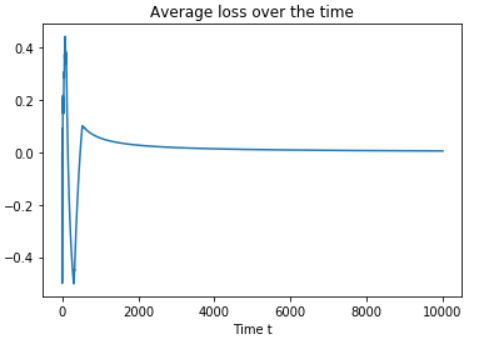
\includegraphics[height=150pt]{image1/q7a_average_loss.png}
      \caption{Average loss as a function of $t$ when playing \lstinline{EXP3} vs \lstinline{EXP3}.}
      \label{fig:q7a}
    \end{subfigure}%
    \hspace{2mm}
    \begin{subfigure}{.47\textwidth}
      \centering
      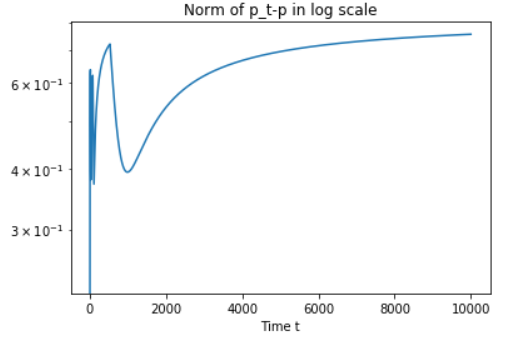
\includegraphics[height=150pt]{image1/q7b_norm_pt.png}
      \caption{Distance between the player's distribution and the uniform distribution.}
      \label{fig:q7b}
    \end{subfigure}%
    \caption{}
    \end{figure}
    
    As a result, when we plot the distance between the player's distribution and the uniform distribution, it does not tend to $0$, as shown in figure \ref{fig:q7b}.

    \end{solution}
\end{enumerate}

\newpage
\paragraph{Optional extentions} The following questions are optional.

\begin{enumerate}[resume]
    \item Repeat Question 4.a) when the adversary is playing a \lstinline{UCB} algorithm. Who wins between \lstinline{UCB} and \lstinline{EXP3}?
    
    \begin{solution}

    \end{solution}
    
    
    \item In the last lecture, we see that EXP3 has a sublinear expected regret. Yet, as shown by question 6.e), it is extremely unstable with a large variance. Implement \lstinline{EXP3.IX} (see Chapter 12 of \cite{lattimore2018bandit}) a modification of \lstinline{EXP3} that controls the regret in expectation and simultaneously keeps it stable. 
    Repeat question 3.e) with \lstinline{EXP3.IX}.
    
    \begin{solution}

    \end{solution}
    
    
    \item Try different games (not necessarily zero-sum games). In particular, how these algorithms behave for the prisoner's dilemna (see wikipedia)? The prisoner's dilemna is a two-player games that shows why two completely rational individuals might not cooperate, even if it appears that it is in their best interests to do so. The losses matrices are:
    \begin{equation*}
    L^{(player)} = \begin{pmatrix}
       1 & 3 \\
       0 & 2 
    \end{pmatrix} \quad \text{and} \quad 
    L^{(adversary)} = \begin{pmatrix}
       1 & 0 \\
       3 & 2 
    \end{pmatrix}  \,.
    \end{equation*}
    
    \begin{solution}

    \end{solution}
\end{enumerate}

\section*{Part 2. Theory -- Sleeping experts}

The classical definition of regret compares the performance of an algorithm with the performance of the best ``constant'' action. But in some applications, some actions may be sometimes unavailable. The purpose of this exercise is to deal with this issue. 

\medskip
We consider the following full-information setting with a finite decision set $\Xcal := \{1,\dots,K\}$. At each time $t\geq 1$, a subset of active decisions $A_t \subseteq \Xcal$ is available, the other decisions are sleeping (or inactive) and cannot be chosen; the player chooses a distribution $p_t$ over active decision $A_t$ (i.e., $\sum_{j \in A_t} p_t(j) = 1$ and $p_t(k) = 0$ for $k \notin A_t$) and observes the loss $\smash{\ell_t(k) \in [0,1]}$ of all decisions in $A_t$. The sleeping regret is defined
\begin{equation}
	\label{eq:sleeping_regret}
	\tag{Sleeping regret}
	R_T(k) := \sum_{t=1}^T \big(p_t \cdot \ell_t - \ell_t(k)\big) \indic\{k \in A_t\} \,,
\end{equation}
with respect to decision $k \in \Xcal$, where $p_t \cdot \ell_t = \sum_{j\in A_t} p_t(j) \ell_t(j)$ is the loss of the player. 
% The goal is to design an algorithm controlling $R_T(k)$ for all $k$.

\begin{enumerate}[resume]
	\item
	{\bfseries The prod algorithm}
	Here, we consider the case where all experts are active $A_t = \Xcal$ for all $t \geq 1$. Let $0\leq \eta(1),\dots,\eta(K)\leq 1/2$ be $K$ parameters. We define the weights 
		\begin{equation}
		    \begin{aligned}
			p_t(k) = \frac{\eta(k) w_t(k)}{\sum_{j=1}^K \eta(j) w_t(j)} \qquad \text{where} \quad &w_t(k) = \prod_{s=1}^{t-1}\Big(1+\eta(k)\big(p_s \cdot \ell_s - \ell_s(k)\big)\Big)\quad \text{if}\  t\geq2\quad \\
			&w_1(k) = 1\,,
			\end{aligned}
			\label{eq:prod}
			\tag{$*$}
		\end{equation}
		
	for all $k \in \Xcal$ and $t \geq 1$.
	\begin{enumerate}[label=(\alph*)]
		\item Prove that $\log(1+x) \geq x - x^2$ for $x \geq -1/2$.
		
        \begin{solution}
        Let $g: x \mapsto \log \br{1 + x} - x + x^2$ defined on $\lc - \frac{1}{2}, + \infty \rp$. This function is differentiable and for $x \geq - \frac{1}{2}$:
        \begin{equation*}
            g'(x) = \frac{1}{1 + x} - 1 + 2x = \frac{x \br{1 + 2x}}{1 + x}
        \end{equation*}
        
        $g'$ is negative for $x \in \br{- \frac{1}{2}, 0}$, null in $x \in \left\{ - \frac{1}{2}, 0 \right\}$ and positive for $x > 0$. 
        
        Hence, for all $x \geq - \frac{1}{2}$, $g(x) \geq g(0)$, \ie $g(x) \geq 0$. Thus,
        \begin{equation*}
            \boxed{\forall x \geq - \frac{1}{2},\, \log \br{1 + x} \geq x - x^2}
        \end{equation*}
        \end{solution}

		\item Denoting $W_{t} = \sum_{k=1}^K w_t(k)$. Prove that for all $k \in \Xcal$
		\begin{equation*}
			\log W_{T+1} \geq \eta(k) \sum_{t=1}^T \big(p_t \cdot \ell_t - \ell_t(k)\big) - (\eta(k))^2 \sum_{t=1}^T \big(p_t \cdot \ell_t  - \ell_t(k)\big)^2
		\end{equation*}

        \begin{solution}
        Let $k \in \Xcal$. As the weights are positive and that $\log$ is nondecreasing, we have:
                \begin{equation*}
                    \log W_{T+1} = \log \br{\sum_{i=1}^K w_{T+1}(i)} \geq \log \br{w_{T+1}(k)}
                \end{equation*}
                First, since $ 0 \leq \eta(k) \leq \frac{1}{2}$ and since the loss is positive, we have : 
                \begin{equation*}
                    \eta(k)\br{p_s \cdot \ell_s - \ell_s(k)} \geq - \ell_s(k)\eta(k) \geq -\eta(k) \geq -\frac{1}{2}
                \end{equation*}
                Besides, using the definition of the weights and the previous question :
                \begin{equation*}
                    \begin{aligned}
                    \log \br{w_{T+1}(k)} &= \log \sqb{\prod_{s=1}^T \br{1 + \eta(k) \sqb{p_s \cdot \ell_s - \ell_s(k)}}} \\
                    &= \sum_{s=1}^T \log \br{1 + \eta(k) \sqb{p_s \cdot \ell_s - \ell_s(k)}} \\
                    &\geq \sum_{s=1}^T \br{\eta(k) \sqb{p_s \cdot \ell_s - \ell_s(k)} - \eta(k)^2 \sqb{p_s \cdot \ell_s - \ell_s(k)}^2} \\
                    &= \eta(k) \sum_{s=1}^T \br{p_s \cdot \ell_s - \ell_s(k)} - \eta(k)^2 \sum_{s=1}^T \br{p_s \cdot \ell_s - \ell_s(k)}^2
                    \end{aligned}
                \end{equation*}
                
                Thus,
                \begin{equation*}
                    \boxed{\forall k \in \Xcal,\, \log W_{T+1} \geq \eta(k) \sum_{s=1}^T \br{p_s \cdot \ell_s - \ell_s(k)} - \eta(k)^2 \sum_{s=1}^T \br{p_s \cdot \ell_s - \ell_s(k)}^2}
                \end{equation*}
        \end{solution}

		\item Show that $W_{t+1} = W_t$ for all $t\geq 1$. What is the value of $\log(W_{T+1})$?

        \begin{solution}
        Let $t \geq 1$. Using the definition of the weights, we have:
                \begin{equation*}
                    \begin{aligned}
                    W_{t+1} &= \sum_{k=1}^K w_{t+1}(k) \\
                    &= \sum_{k=1}^K w_t(k) \sqb{1 + \eta(k) \br{p_t \cdot \ell_t - \ell_t(k)}} \\
                    &= W_t + \br{p_t \cdot \ell_t} \sum_{k=1}^K w_t(k) \eta(k) - \sum_{k=1}^K w_t(k) \eta(k) \ell_t(k)
                    \end{aligned}
                \end{equation*}
                We denote $\wb_t = \br{w_t(1), \dots, w_t(K)}^\top$ and $\etab = \br{\eta(1), \dots, \eta(K)}^\top$. By definition of $p_t(k)$ for all $k$,
                \begin{equation*}
                    \begin{aligned}
                    W_{t+1} &= W_t + \br{p_t \cdot \ell_t} \br{\wb_t^\top \etab} - \sum_{k=1}^K \br{\wb_t^\top \etab} p_t(k) \ell_t(k) \\
                    &= W_t + \br{p_t \cdot \ell_t} \br{\wb_t^\top \etab} - \br{p_t \cdot \ell_t} \br{\wb_t^\top \etab} \\
                    &= W_t
                    \end{aligned}
                \end{equation*}
                
                Hence,
                \begin{equation*}
                    \boxed{\forall t \geq 1,\, W_{t+1} = W_t}
                \end{equation*}
                
                We can deduce $W_{T+1} = W_1 = K$ and:
                \begin{equation*}
                    \boxed{\log W_{T+1} = \log K}
                \end{equation*}
        \end{solution}

		\item Assuming $\eta(k)$ are well-optimized, show the regret bound for all arms $k \in [K]$
		\begin{equation*}
		\sum_{t=1}^T p_t \cdot \ell_t - \ell_t(k) \leq 2 \sqrt{ (\log K) \sum_{t=1}^T  \big(p_t \cdot \ell_t - \ell_t(k)\big)^2} \,.
		\end{equation*}

        \begin{solution}
        Let $k \in \Xcal$. Using the two previous questions,
                \begin{equation*}
                    \eta(k) \sum_{s=1}^T \br{p_s \cdot \ell_s - \ell_s(k)} \leq \log K + \eta(k)^2 \sum_{s=1}^T \br{p_s \cdot \ell_s - \ell_s(k)}^2
                \end{equation*}
                
                We assume $\eta(k) \neq 0$:
                \begin{equation*}
                    \sum_{s=1}^T \br{p_s \cdot \ell_s - \ell_s(k)} \leq \frac{1}{\eta(k)} \log K + \eta(k) \sum_{s=1}^T \br{p_s \cdot \ell_s - \ell_s(k)}^2
                \end{equation*}
                
                Let $\alpha \in \R$ and $g: x \mapsto \frac{1}{x} \log K + \alpha x$. $g$ is differentiable and for all $x \neq 0$ $g'(x) = \alpha - \frac{1}{x^2} \log K$. $g'$ is null in $x^* = \sqrt{\frac{\log K}{\alpha}}$, negative before and then positive, which shows this is a minimum. We have $g \br{x^*} = 2 \sqrt{\alpha \log K}$. Thus,
                \begin{equation*}
                    \boxed{\forall k \in \Xcal,\, \sum_{t=1}^T \br{p_t \cdot \ell_t - \ell_t(k)} \leq 2 \sqrt{\br{\log K} \sum_{t=1}^T \br{p_t \cdot \ell_t - \ell_t(k)}^2}}
                \end{equation*}
        \end{solution}
    \end{enumerate}

	\item {\bfseries Sleeping experts} 
	Now, we assume that some decisions are sometimes not possible (sleeping), i.e., $A_t \subsetneq \Xcal$ for some $t\geq 1$. The idea is to use Algorithm~\eqref{eq:prod} with past modified losses
	\begin{equation*}
		\tilde \ell_t(k) := \left\{ \begin{array}{ll} \ell_t(k) & \text{if} \ k \in A_t \\ p_t \cdot \ell_t = \sum_{k \in A_t} p_t(k) \ell_t(k) & \text{if} \ k \notin A_t \end{array} \right.\,\,,
	\end{equation*}
	i.e., by assigning the loss of the algorithm $p_t \cdot \ell_t$ to all inactive decisions $k \notin A_t$.
	The algorithm outputs weights $\tilde p_t(k)$ and $\tilde w_t(k)$ obtained by replacing $\ell_t(k)$ with $\tilde \ell_t(k)$ in Equation~\eqref{eq:prod}. This vector is then used to form another weight vector
	\begin{equation*}
		p_t(k) = \frac{\tilde p_t(k) \indic_{k\in A_t}}{\sum_{j=1}^K \tilde p_t(j) \indic_{j \in A_t}}
	\end{equation*}
	which has non zero weights only on active arms $A_t$.

	\begin{enumerate}[label=(\alph*)]
 		\item Show that the instantaneous regret on the modified losses equals the sleeping regret on the original rewards; i.e. for all $t\geq 1$, and all $k \in \Xcal$
		\begin{equation*}
			 \tilde p_t \cdot \tilde \ell_t - \tilde \ell_t(k)  = \big(p_t \cdot \ell_t - \ell_t(k)\big) \indic_{k \in A_t} \,.
		\end{equation*}
		
		\begin{solution}
		Let $t \geq 1$. We first note that as $p_t$ has nonzero weights only on active arms, we have:
        \begin{equation*}
            p_t \cdot \ell_t = \sum_{k \in A_t} p_t(k) \ell_t(k) = \sum_{k=1}^K p_t(k) \ell_t(k) \mathds{1}_{k \in A_t} = \sum_{k=1}^K p_t(k) \ell_t(k)
        \end{equation*}
        
        Let $k \in \Xcal$. By definition of $\tilde{p}_t$ and $\tilde{\ell}_t$:
        \begin{equation*}
            \begin{aligned}
            \tilde{p}_t \cdot \tilde{\ell}_t &= \sum_{i=1}^K \tilde{p}_t(i) \tilde{\ell}_t(i) \\
            &= \sum_{i=1}^K \tilde{p}_t(i) \br{\ell_t(i) \mathds{1}_{i \in A_t} + \br{p_t \cdot \ell_t} \mathds{1}_{i \in A_t^c}} \\
            &= \sum_{i=1}^K \br{\sum_{j=1}^K \tilde{p}_t(j) \mathds{1}_{j \in A_t}} p_t(i) \ell_t(i) + \br{p_t \cdot \ell_t} \sum_{i=1}^K \tilde{p}_t(i) \mathds{1}_{i \in A_t^c} \\
            &= \br{p_t \cdot \ell_t} \br{\sum_{j=1}^K \tilde{p}_t(j) \mathds{1}_{j \in A_t} + \sum_{i=1}^K \tilde{p}_t(i) \mathds{1}_{i \in A_t^c}} \\
            &= p_t \cdot \ell_t
            \end{aligned}
        \end{equation*}
        
        Besides, $\tilde{\ell}_t(k) = \ell_t(k) \mathds{1}_{k \in A_t} + \br{p_t \cdot \ell_t} \mathds{1}_{k \in A_t^c}$. Thus,
        \begin{equation*}
            \boxed{\forall k \in \Xcal,\, \tilde{p}_t \cdot \tilde{\ell}_t - \tilde{\ell}_t(k) = \br{p_t \cdot \ell_t - \ell_t(k)} \mathds{1}_{k \in A_t}}
        \end{equation*}
		\end{solution}
		
		
		\item Conclude that $R_T(k) \leq 2 \sqrt{(\log K)T_k}$ where $T_k = \sum_{t=1}^T \indic\{k\in A_t\}$ is the number of times arm $k$ is active.
		
		\begin{solution}
	Let us recall the definition of  $\tilde \ell_t(k)$	\begin{equation*}
		\tilde \ell_t(k) := \left\{ \begin{array}{ll} \ell_t(k) & \text{if} \ k \in A_t \\ p_t \cdot \ell_t = \sum_{k \in A_t} p_t(k) \ell_t(k) & \text{if} \ k \notin A_t \end{array} \right.\,\,,
	\end{equation*}
Since $l_t(k) \in [0,1]$,  $\tilde \ell_t(k) \in [0,1]$, and since $\Tilde{p}_t$ and $\Tilde{w}_t$ are constructed as in 11, we can apply the results of question 11. Besides, we have $\br{p_t \cdot \ell_t - \ell_t(k)} \leq 1$. Thus, $ \forall k \in \Xcal $ :
\begin{equation*}
    \begin{aligned}
    \sum_{t=1}^T \br{\tilde{p}_t \cdot \tilde{\ell}_t - \tilde{\ell}_t(k)} &\leq 2 \sqrt{\br{\log K} \sum_{t=1}^T \br{p_t \cdot \tilde{\ell}_t - \tilde{\ell}_t(k)}^2}\\
    & \leq 2 \sqrt{\br{\log K} \sum_{t=1}^T \br{\br{p_t \cdot \ell_t - \ell_t(k)}\mathds{1}_{k \in A_t}}^2} \\
    & \leq 2 \sqrt{\br{\log K} \sum_{t=1}^T \mathds{1}_{k \in A_t}}\\
    & \leq 2 \sqrt{\br{\log K}T_k}
    \end{aligned}
\end{equation*}
Thus : 
 \begin{equation*}
                    \boxed{\forall k \in \Xcal,\, \sum_{t=1}^T \br{p_t \cdot \tilde{\ell}_t - \tilde{\ell}_t(k)} \leq 2 \sqrt{\br{\log K}T_k}}
                \end{equation*}


		\end{solution}
		
	\end{enumerate}
\end{enumerate}

\section*{Part 3. Experiments -- predict votes of surveys}

In these experiments, we will apply online convex optimization algorithms to pairwise comparison datasets. Comparison data arises in many different applications such as sport competition, recommender systems or web clicks. We consider the following sequential setting. Let $\Zcal = \{1,\dots,N\}$ be a finite set of items (for example football teams in a competition).

\medskip
At each iteration $t\geq 1$, 
\begin{itemize}[topsep=-2pt]
	\item the learner receives the labels of two items that are competing $z_t = (z_t(1),z_t(2)) \in \Zcal^2$
	\item the learner predicts $\hat y_t \in (0,1)$ the probability of victory of item $z_t(1)$. 
	\item the environment reveals the result of the match $y_t = 1$ if item $z_t(1)$ wins the match and $y_t = 0$ otherwise (if team $z_t(2)$ wins).
\end{itemize}
The learner aims at minimizing his cumulative loss: $\hat L_T = \sum_{t=1}^T \ell(\hat y_t,y_t)$, where 
$
	\ell(\hat y_t,y_t) = (1-\hat y_t) y_t + \hat y_t (1-y_t) 
$.

\begin{enumerate}[resume]
	\item Justify the choice of $\ell$.

\begin{solution}
When dealing with a classification problem like this one, a natural choice would be to minimize the cross-entropy. However, because the definition involves a logarithm, this loss may not be smooth enough for the algorithms we want to use, such as the Online Gradient Descent which requires the loss to have a bounded gradient. Hence, we use a similar but smoother loss, as defined above, to solve this classification problem.
\end{solution}
\end{enumerate}


	\paragraph{Datasets} We consider two datasets from~\cite{salganik2015wiki} that contain surveys of civic comparisons (can be download at \url{http://pierre.gaillard.me/teaching/mva}). Each dataset consists of two files of $T=15\,000$ rows corresponding to votes:
	\begin{itemize}
		\item ideas dataset: the participants are suggested two politic ideas such as ('free beer' vs 'free ice cream') and are asked to vote for the best. 
		\item politicians dataset: the participants are asked  which political figure within a pair such as ('Obama' vs 'Goldman Sachs') had ``the worse year in Washington.''
	\end{itemize}
	The datasets contain two files: 
	\begin{itemize}
		\item \texttt{ideas-id.csv} (resp. \texttt{politicans-id.csv}) that contains id and text of the ideas (resp. political figures). 
		\item \texttt{ideas-votes.csv} (resp. \texttt{politicians-votes.csv}) that contains the id of the two competing ideas (resp. political figures) in z1 and z2 and a column $y$ which is 1 if the participant voted for z1 and 0 otherwise.
	\end{itemize}
	The goal of the learner is to sequentially predict the results of the votes minimizing the number of mistakes.

\begin{enumerate}[resume]
	\item Implement the Exponentially Weighted Average Forecaster (EWA) and Online Gradient Descent (OGD) (and optionally the Prod forecaster of question 1)  with parameter $\eta >0$ that at each round $t\geq 1$ take a finite set of predictions $f_t(1),\dots, f_t(K) \in [0,1]^K$ and forecast $\hat y_t = \sum_{k=1}^K p_t(k) f_t(k) \in [0,1]$ the probability that idea 1 wins the vote. \footnote{This question does not require any answer in the final report. $f_t(1),\dots,f_t(K)$ are prediction of experts that are inputs, they will be defined explicitely in the next question.}

	For the euclidean projection onto the simplex, see~\cite{duchi2008efficient}.

\begin{solution}
 See the code for the implementation details.  
\end{solution}

	\item We consider the sleeping strategies indexed by $k \in \{1,\dots,2N\}$ that predict for $1\leq k\leq N$
	\begin{equation*}
		 \qquad f_t(k) = \left\{ 
			\begin{array}{cc}
				1 & \text{if } k = z_t(1) \\
				0 & \text{if } k = z_t(2) \\
				\emptyset & \text{otherwise}
			\end{array}
		\right. \qquad \text{and} \qquad f_t(k+N) =  \left\{ 
			\begin{array}{cc}
				0 & \text{if } k = z_t(1) \\
				1 & \text{if } k = z_t(2) \\
				\emptyset & \text{otherwise}
			\end{array}
		\right. \,,
	\end{equation*}
	where $\emptyset$ means that the strategy is sleeping.
	Basically, $f_t(k)$ (resp. $f_t(k+N)$) predicts always the victory (resp. loss) of the idea $k$ during the votes. Remark that the sleeping trick of question 2) works for any algorithm so that we might replace $\emptyset$ with the prediction of the algorithm itself $\hat y_t$. Run the two algorithms of the preceding question (EWA, OGD) with these predictions  $f_t(1),\dots, f_t(K) \in [0,1]^K$. 

	\begin{enumerate}[label=(\alph*)]
		\item Plot the cumulative loss of the algorithms at $T = 15\,000$ according to different values of $\eta \in (0,1/2)$ chosen in a grid.
	
	In this question, we plot the cumulative loss for different values of $\eta$, computes with the OGD update and the EWA update.
	
	\begin{solution}
	    \begin{figure}[h!]
    \centering
    \begin{subfigure}{.47\textwidth}
      \centering
      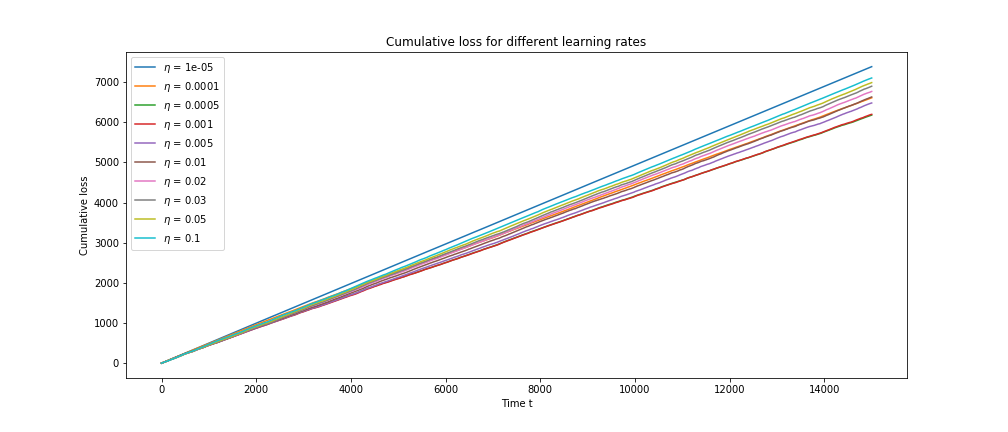
\includegraphics[height=110pt]{image1/image2/VOTES_OGD_cumulative_loss.png}
      \caption{Cumulative loss when playing OGD for different $\eta$ values}
      \label{fig:q7a}
    \end{subfigure}%
    \hspace{2mm}
    \begin{subfigure}{.47\textwidth}
      \centering
      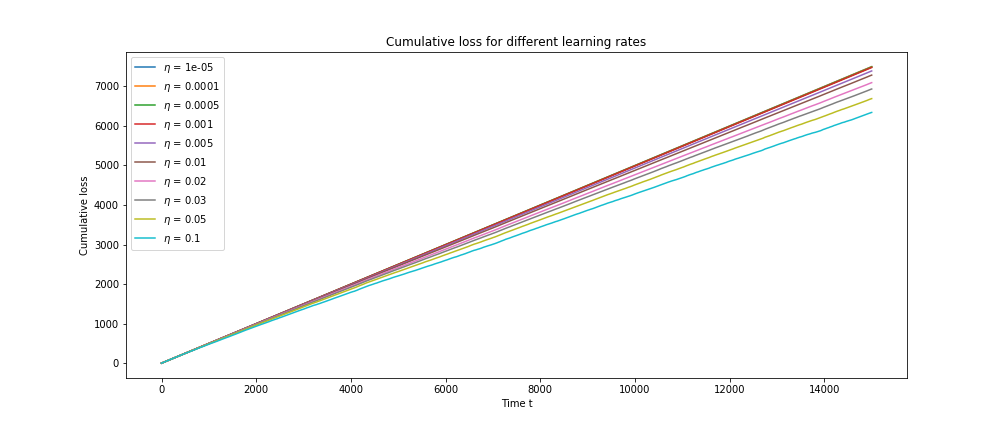
\includegraphics[height=110pt]{image1/image2/VOTES_EWA_cumulative_loss.png}
      \caption{Cumulative loss when playing EWA for different $\eta$ values}
      \label{fig:q7b}
    \end{subfigure}%
    \caption{}
    \end{figure}
	\end{solution}

In both case, the best cumulative loss is obtained for $\eta = 0.001$. However, it is not the value of $\eta = \sqrt{\frac{log(K)}{T}}=0.02$ for which the regret has an optimal bound. Lower and higher values for $\eta$ increases the cumulative loss.

		\item Plot the average expected loss of the algorithms $(1/t)\hat L_t$ according to the number of rounds $t=1,\dots,T$ (i.e., number of votes) for well-chosen values of $\eta$ (justify the choice). Do the algorithms beat random predictions?
	Based on the observation of question a), we choose $\eta=0.001$ for the next plots.
	
		\begin{solution}
	    \begin{figure}[h!]
    \centering
    \begin{subfigure}{.47\textwidth}
      \centering
      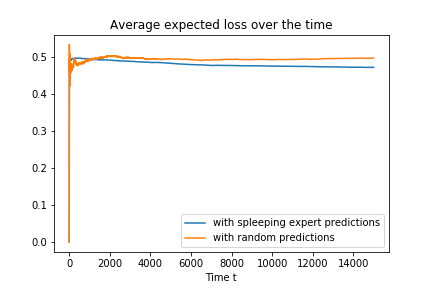
\includegraphics[height=130pt]{image1/image2/VOTES_random_EWA.png}
      \caption{Average loss when playing EWA for $\eta=0.001$, compared with random predictions}
      \label{fig:q7a}
    \end{subfigure}%
    \hspace{2mm}
    \begin{subfigure}{.47\textwidth}
      \centering
      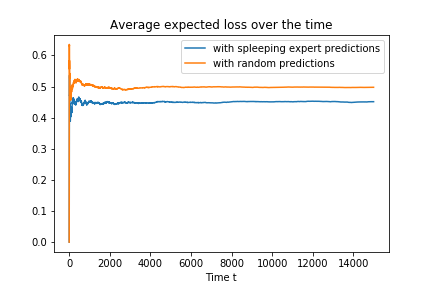
\includegraphics[height=130pt]{image1/image2/VOTES_random_OGD.png}
      \caption{Average loss when playing OGD for $\eta=0.001$, compared with random predictions}
      \label{fig:q7b}
    \end{subfigure}%
    \caption{}
    \end{figure}

EWA produces a slightly better prediction when compared with the average loss of the random prediction. Its accuracy is around 62\%. OGD produces a much better solution in terms of average loss, from the beginning, and that has an accuracy around 60 \%.
	\end{solution}

		\item At each round $t\geq 1$, assume that the algorithms predict the vote $\hat Y_t = 1$ with probability $\hat y_t$ and $0$ otherwise. For each algorithm (for the $\eta$ chosen in question 6(a)), plot its true average loss 
		\begin{equation*}
			\textstyle{\frac{1}{t} \sum_{s=1}^t \indic_{\hat Y_s \neq y_s} \,,}
		\end{equation*}
		according to $t=1,\dots,T$.
		
		\begin{solution}
		\begin{figure}[h!]
    \centering
    \begin{subfigure}{.47\textwidth}
      \centering
      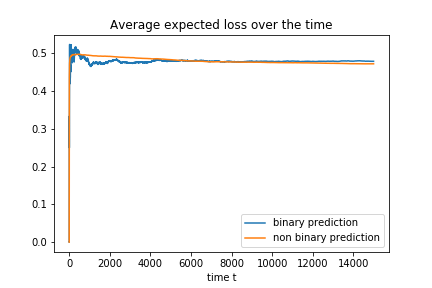
\includegraphics[height=130pt]{image1/image2/VOTES_EWA_bernoulli.png}
      \caption{Average loss when playing EWA for $\eta=0.001$, compared with binary predictions}
      \label{fig:q7a}
    \end{subfigure}%
    \hspace{2mm}
    \begin{subfigure}{.47\textwidth}
      \centering
      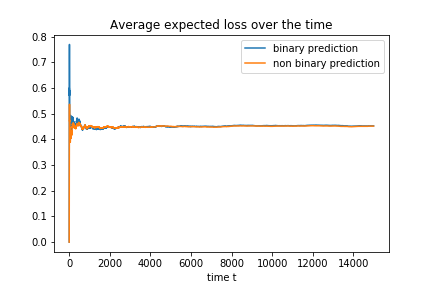
\includegraphics[height=130pt]{image1/image2/VOTES_OGD_bernoulli.png}
      \caption{Average loss when playing OGD for $\eta=0.001$, compared with binary predictions}
      \label{fig:q7b}
    \end{subfigure}%
    \caption{}
    \end{figure}
		\end{solution}
	Even if the true average is a dirac, which is non convex and whose gradient is not bounded, its loss is almost the same as the loss from question 14), for both updates. 

	\end{enumerate}

	\item (optional) Explore different ideas to improve the final performance. For example, you can add new sleeping strategies to be combined or you can perform OGD or EG to estimate the best Bradley Terry model (\url{https://en.wikipedia.org/wiki/Bradley-Terry_model}) on the fly,\dots
\end{enumerate}

\bibliographystyle{plain}
\bibliography{biblio}

\end{document}
